%%
% The BIThesis Template for Bachelor Graduation Thesis
%
% 北京理工大学毕业设计(论文)附录 —— 使用 XeLaTeX 编译
%
% Copyright 2020-2022 BITNP
%
% This work may be distributed and/or modified under the
% conditions of the LaTeX Project Public License, either version 1.3
% of this license or (at your option) any later version.
% The latest version of this license is in
%   http://www.latex-project.org/lppl.txt
% and version 1.3 or later is part of all distributions of LaTeX
% version 2005/12/01 or later.
%
% This work has the LPPL maintenance status `maintained'.
%
% The Current Maintainer of this work is Feng Kaiyu.
%
% Compile with: xelatex -> biber -> xelatex -> xelatex

\begin{appendices}
\section{更多实验结果}


为了更好地证明我们的模型性能,我们在图\ref{fig:supp-time-pose-function-qualitative}中定性地显示了我们估计的轨迹和真实轨迹之间的差异。

\begin{figure}[p]
    \centering
    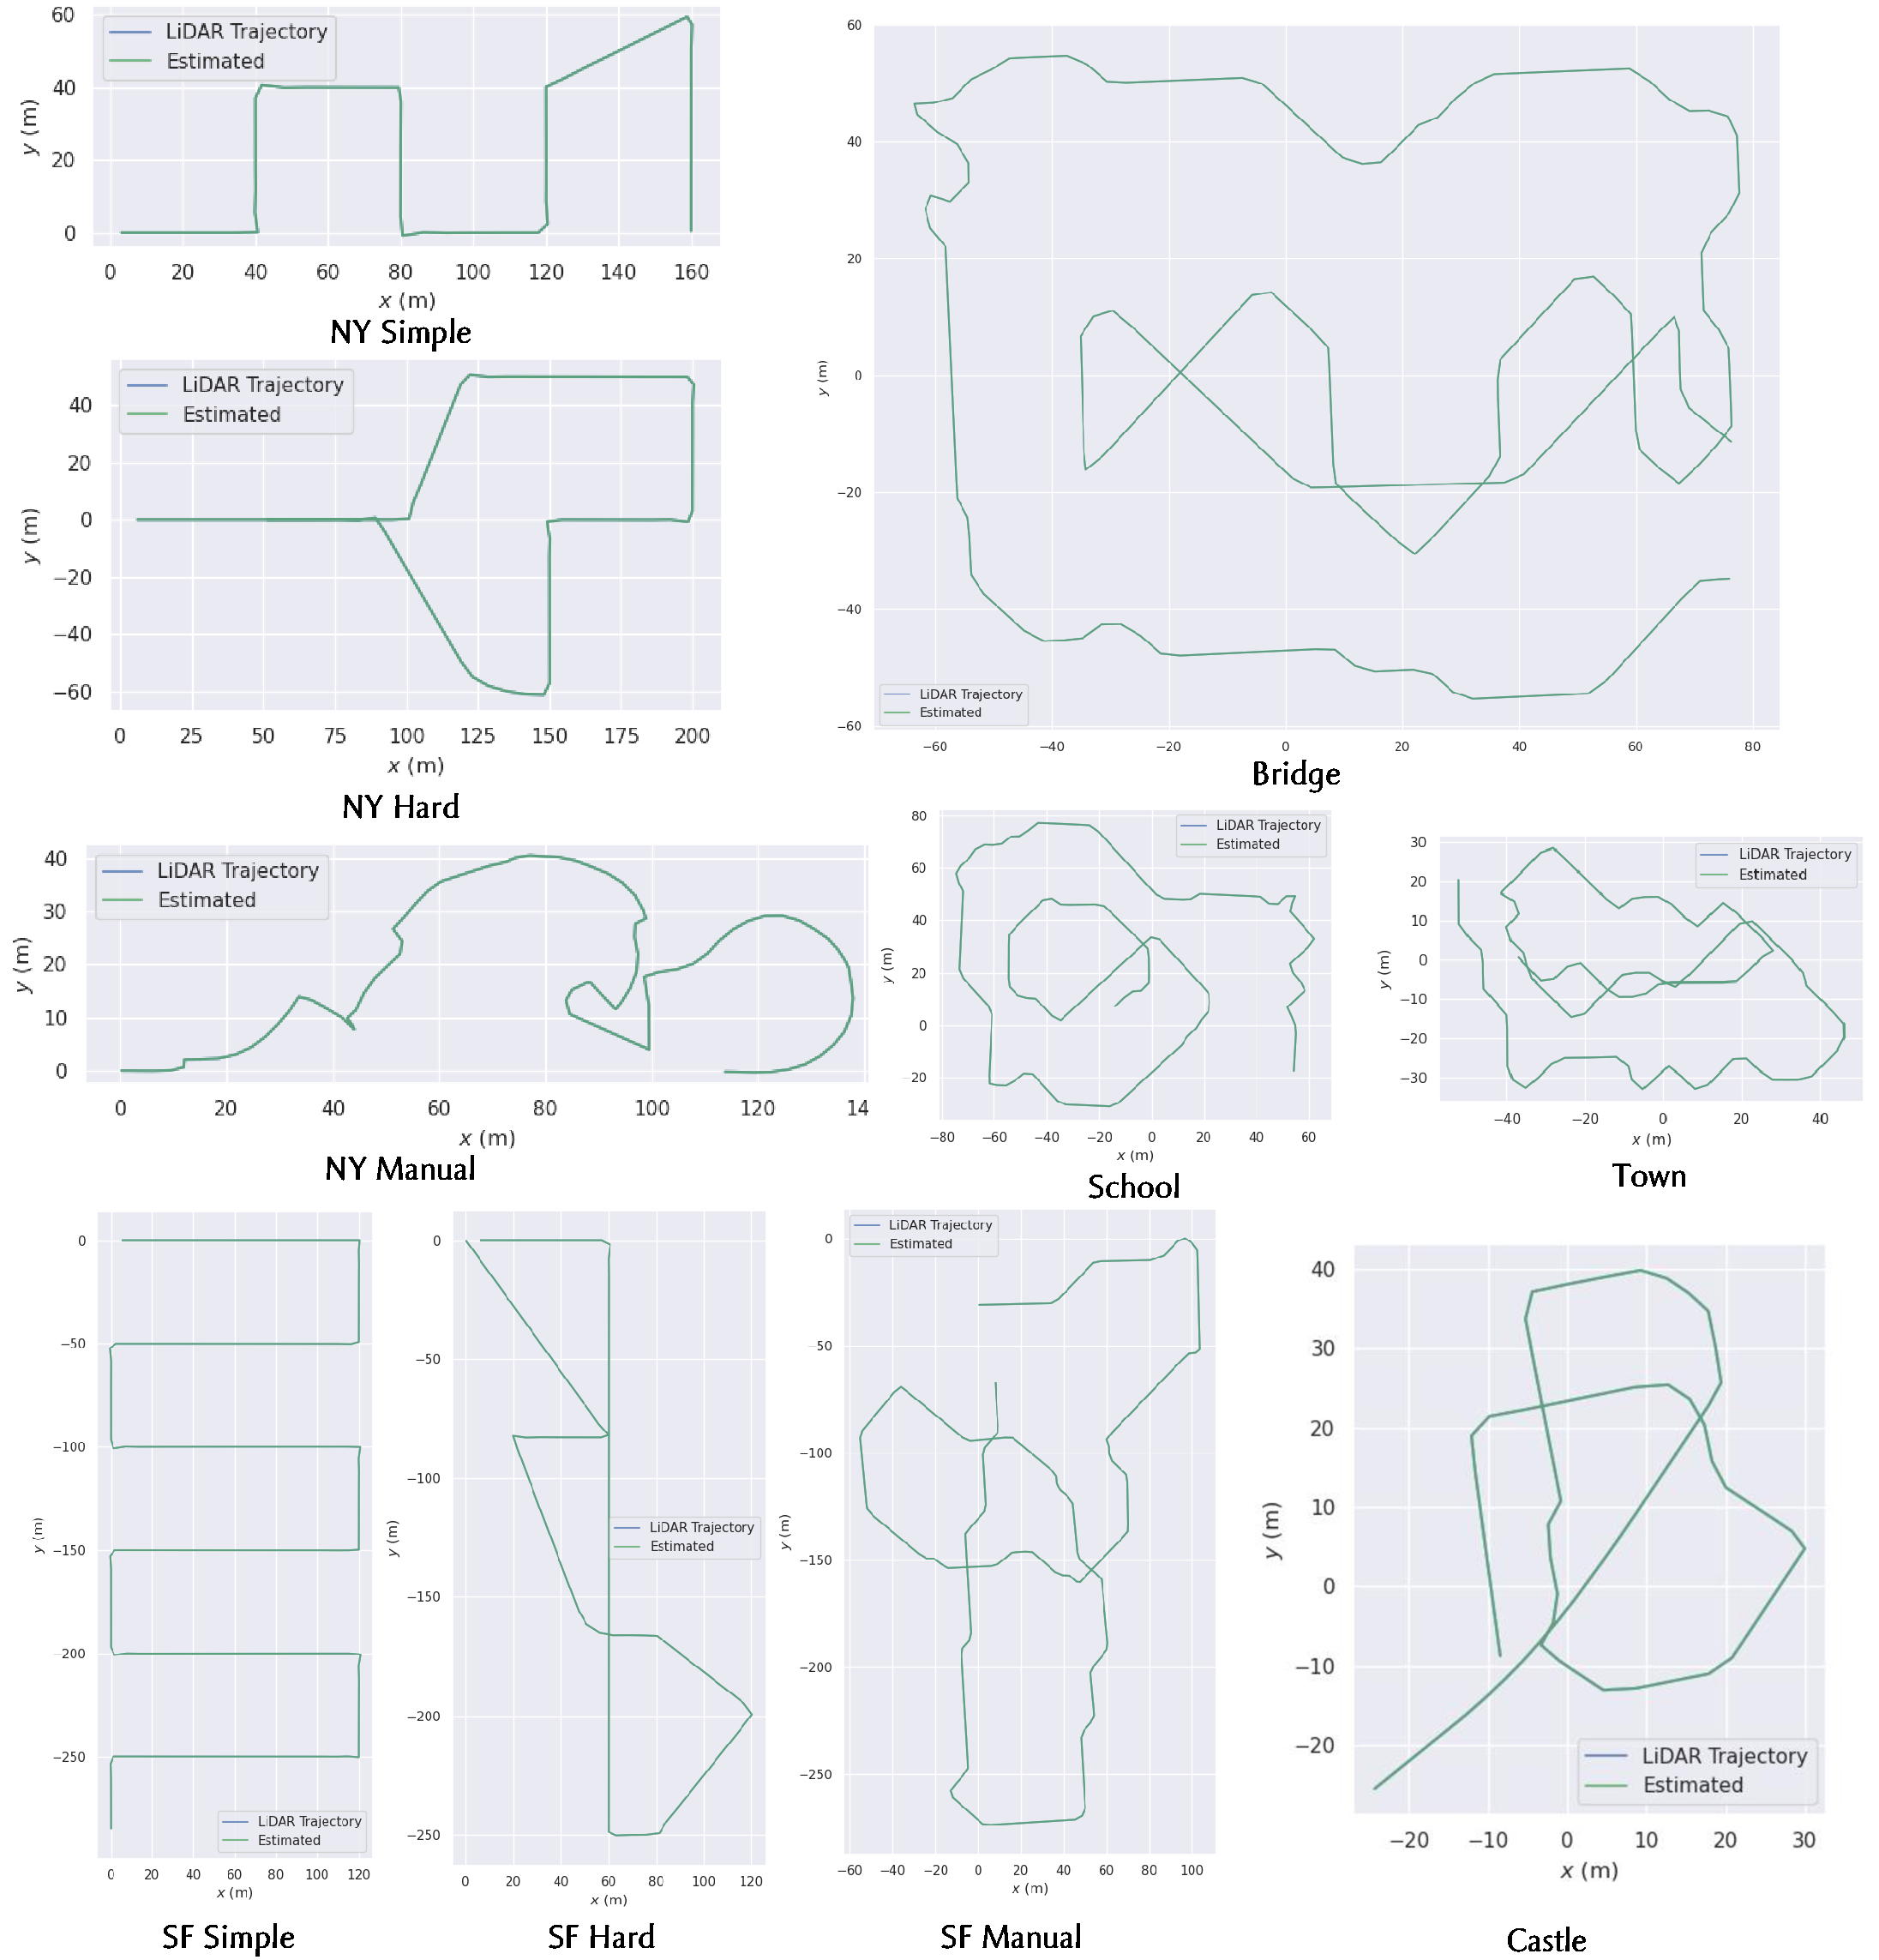
\includegraphics[width=\textwidth]{undergraduate-thesis/images/time-pose function/evo.pdf}
    \caption{TPF函数在AUS数据集上的定性实验结果}
    \label{fig:supp-time-pose-function-qualitative}
\end{figure}

\section{数据集示例}

本文所提出的AUS数据集是使用模拟器在已经建立的几个城市场景模型\cite{ArtStation, lin_capturing_2022}上收集的。本文用虚拟无人机沿着给定的路径穿过场景,从俯视图中拍摄了场景的RGB照片和深度图。图\ref{fig:supp-example}中展示了一些捕获的图像及其时间戳。
由于模拟器的输出是密集的RGB图像和深度图,本文在训练期间将密集的深度图随机下采样到更稀疏的深度图,以更好地模拟真实的无人机射击数据,在评估过程中,使用真实深度图来计算模型深度预测的评估指标。

\begin{figure}[htbp]
    \centering
    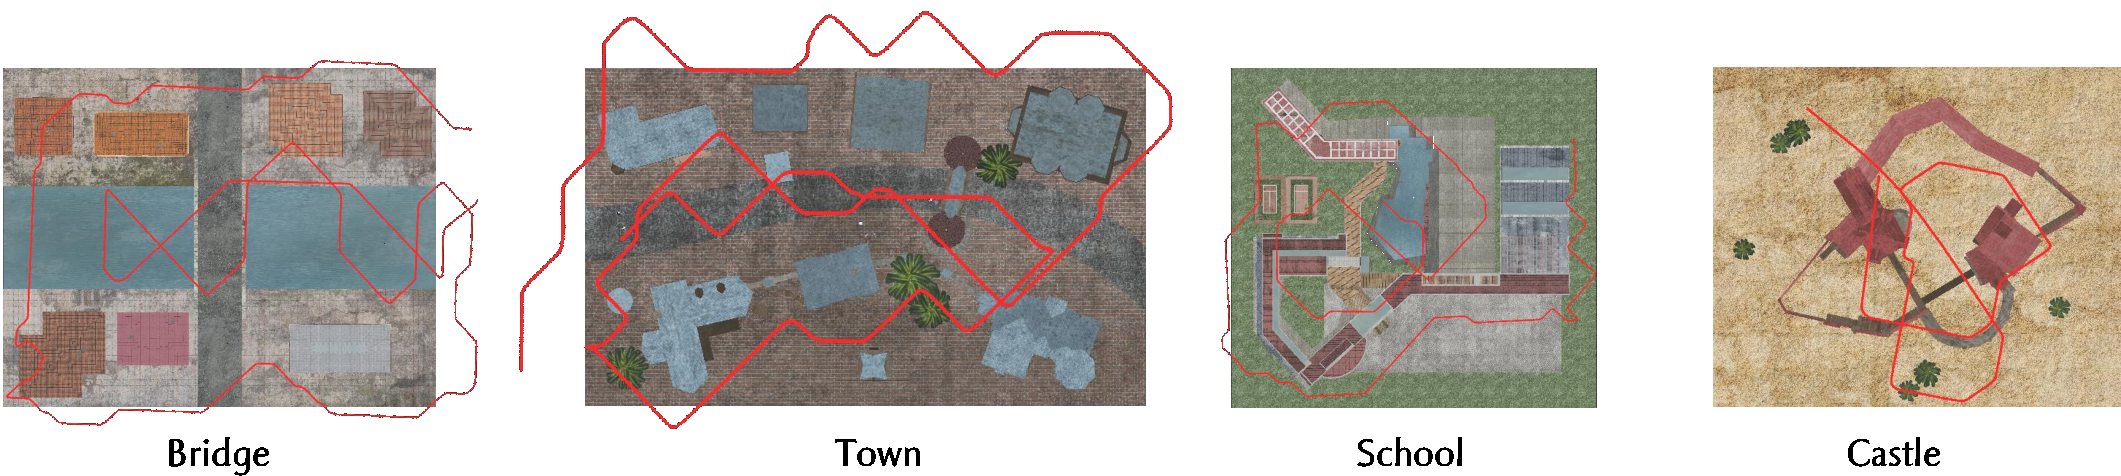
\includegraphics[width=0.9\textwidth]{undergraduate-thesis/images/time-pose function/virtual-top-view.pdf}
    \caption{AUS虚拟场景中覆盖的轨迹的俯视图。}
    \label{fig:virtual-top-view}
\end{figure}

\begin{figure}[htbp]
    \centering
    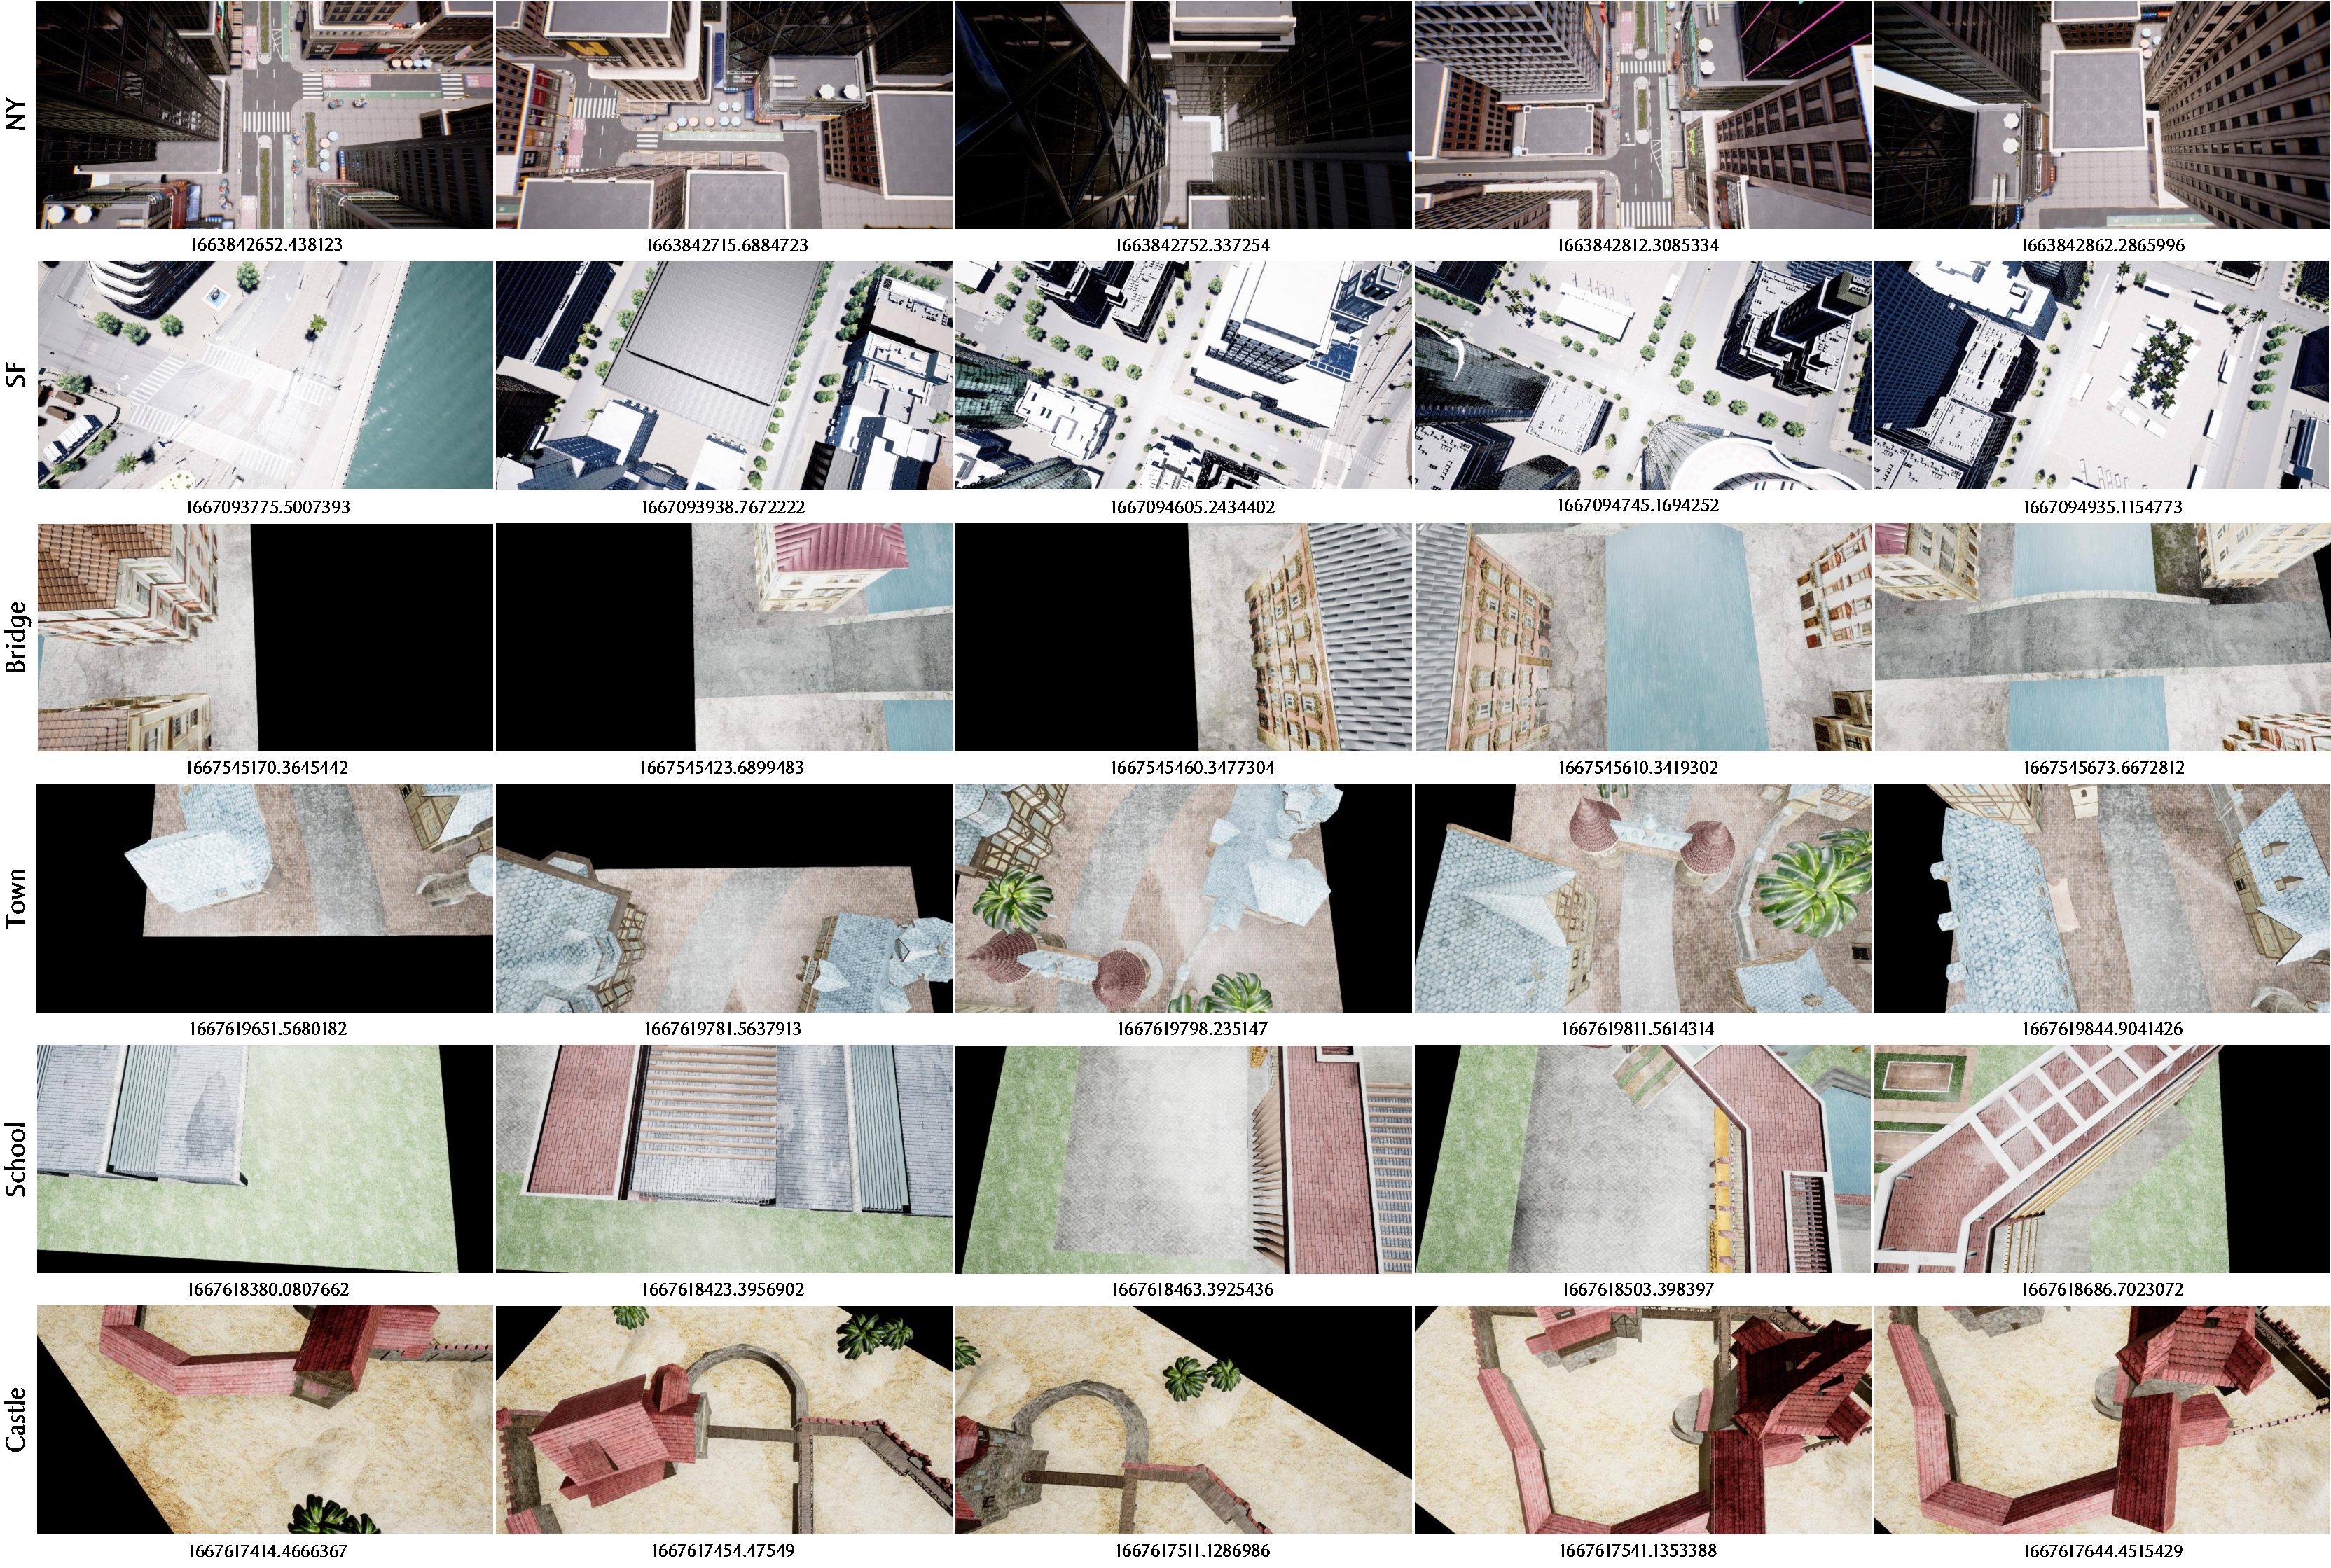
\includegraphics[width=\textwidth]{undergraduate-thesis/images/time-pose function/data-example.pdf}
    \caption{RGB图像和每个AUS轨迹中对应的时间戳。}
    \label{fig:supp-example}
\end{figure}

\begin{figure}[htbp]
    \centering
    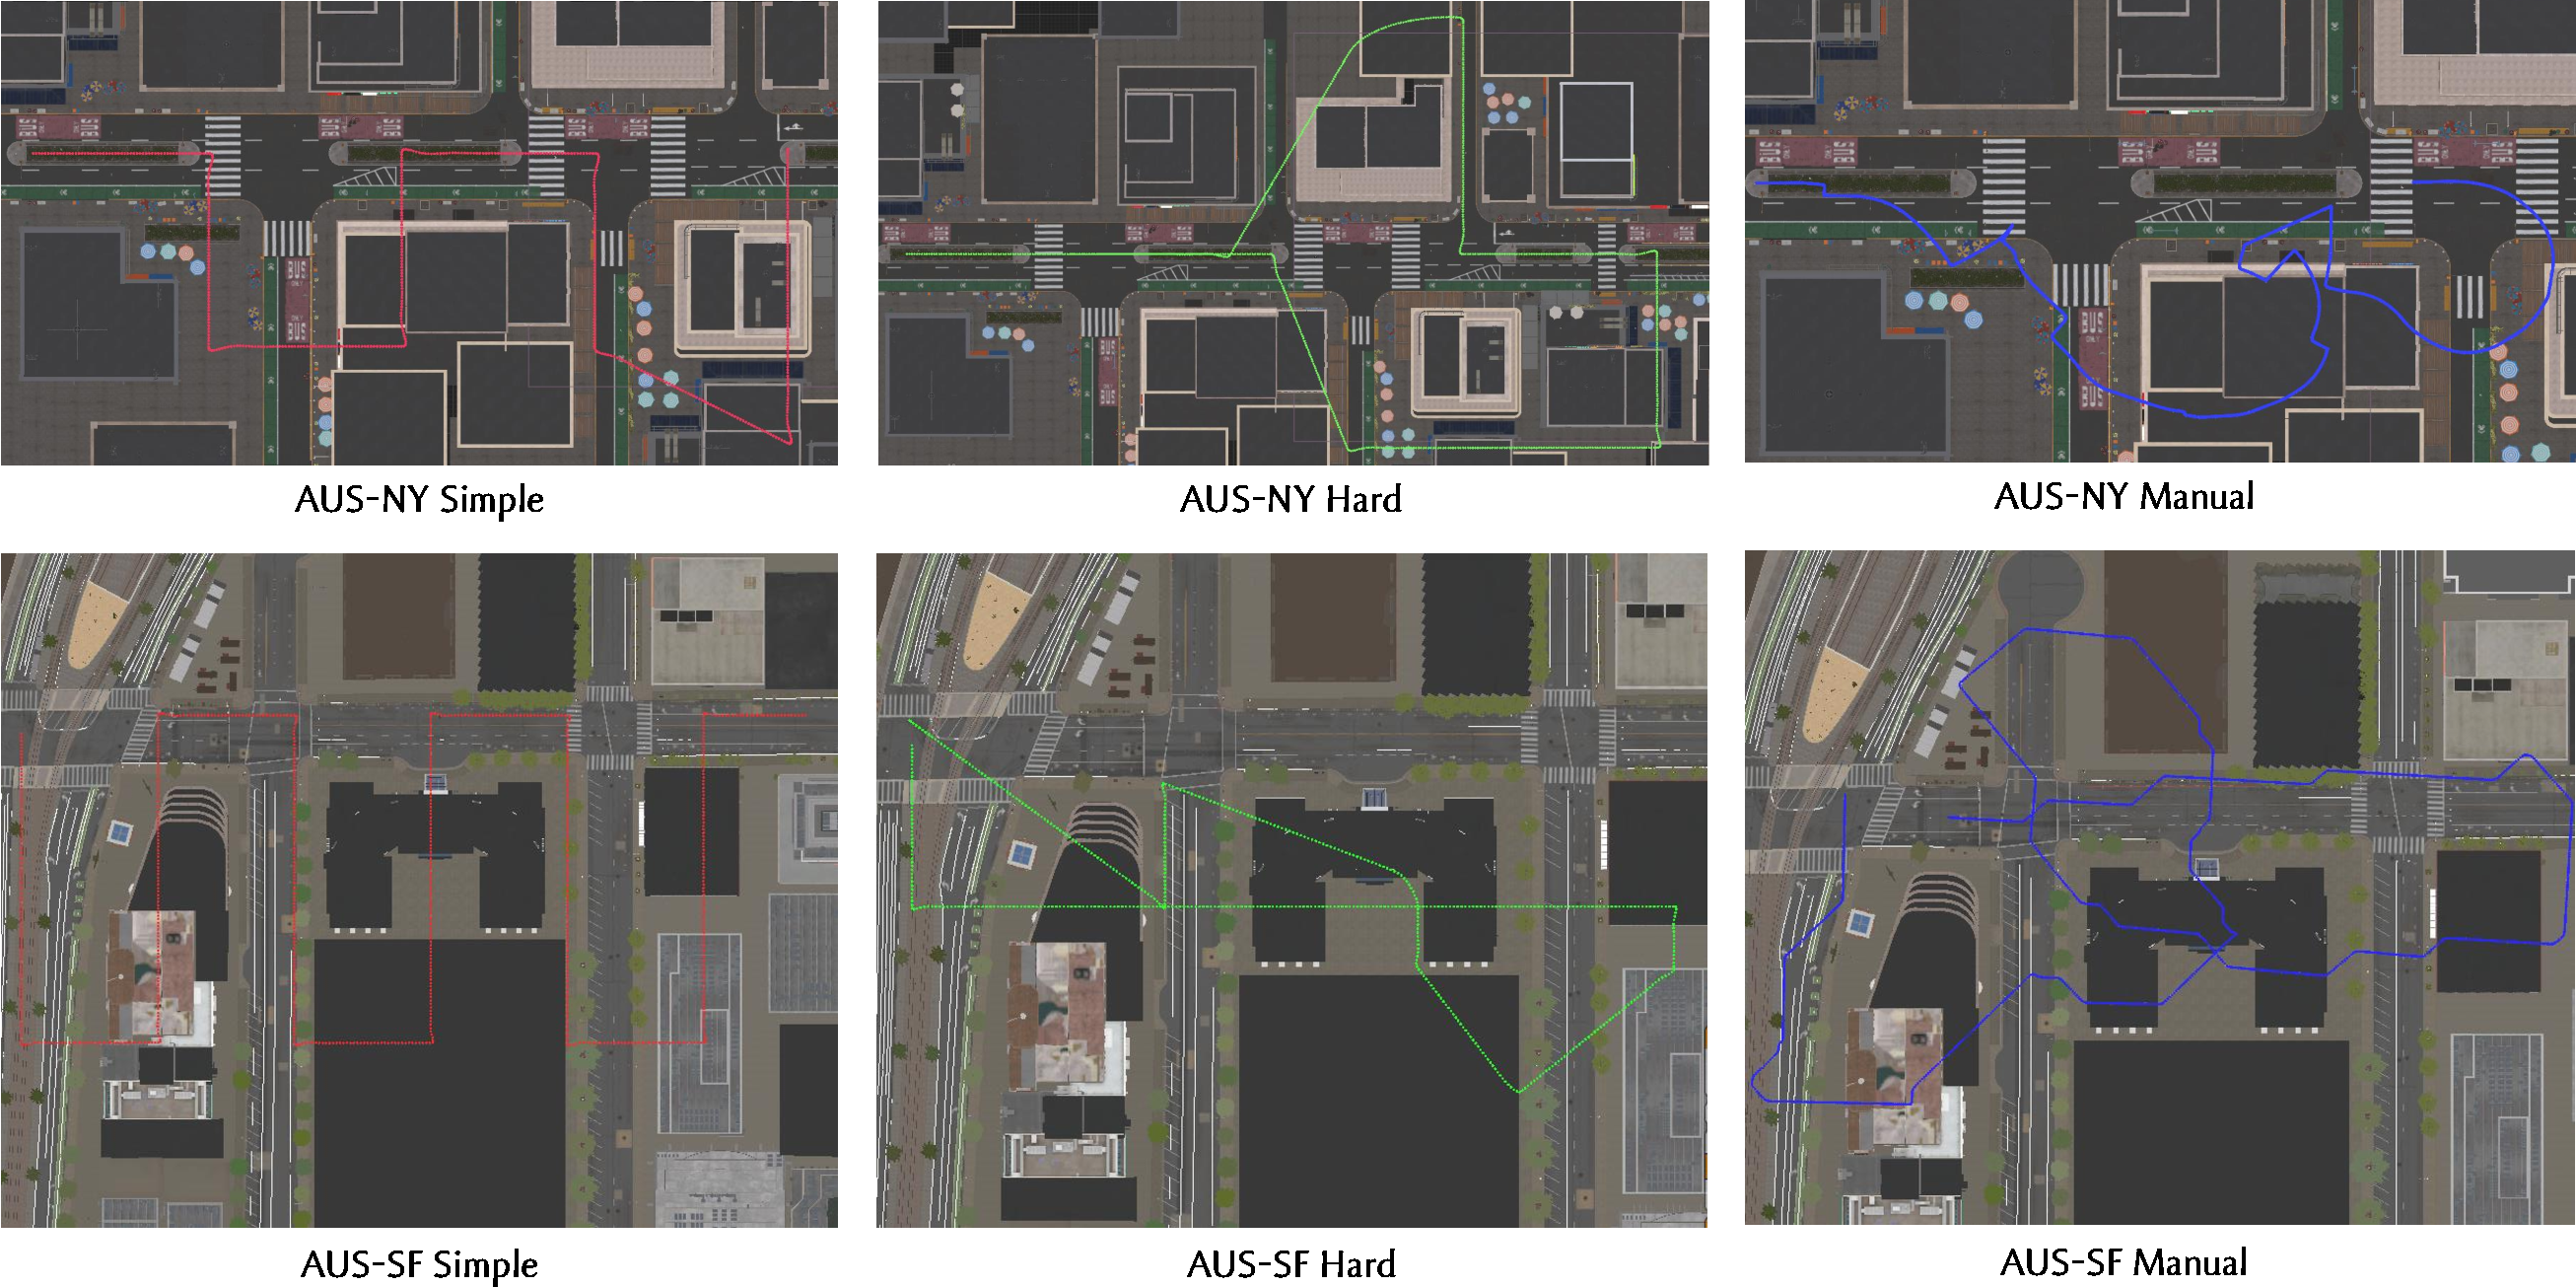
\includegraphics[width=\textwidth]{undergraduate-thesis/images/time-pose function/city-top-view.pdf}
    \caption{AUS-NY和AUS-SF中涵盖的轨迹的俯视图。}
    \label{fig:supp-city-top-view}
\end{figure}




\section{散射效应公式推导过程}
第\ref{chapter: real-world data}章中使用多个隐式函数来帮助理解深度-辐射协方差损失,这一节提供部分推到过程。

定理 \ref{thm:radiance}展示了任意表面上一点$\mathbf P_1$的辐射颜色与带雾距离 $t_\text{haze\:i}$ 是独立随机变量。 

\begin{theorem}
对任意表面上的一点$\mathbf P_1$ ,$\partial\mathbf{Radiance}/\partial t_\text{haze\:i} = 0$  。
\label{thm:radiance}
\end{theorem}
\begin{proof}  由于
\begin{align*}
\hat\sigma(t)&=\sigma(\mathbf{O}_i+t\cdot\mathbf d_i)\\
&=\sigma(\mathbf P_1 + (t-t_\text{haze\:i})\cdot\mathbf d_i),\\
\hat{\mathbf c}(t) &= \mathbf c(\mathbf P_1 + (t-t_\text{haze\: i})\cdot\mathbf{d}_i,\mathbf d_i), and\\
T'(t) &= \exp(-\int_{t_\text{haze\:i}}^t\hat\sigma(\tau)\text d\tau)\\
&=\exp(-\int_{0}^{t-t_\text{haze\:i}                    }\sigma(\mathbf P_1 + \tau'\cdot \mathbf d_i)\text d\tau'),
\end{align*}
因此: 

\begin{align*}
    &\qquad\mathbf{Radiance}(\mathbf{d}_i, \mathbf P_1, t_\text{haze\: i})\\
     &= \int_{t_\text{haze\: i}}^\infty T'(t)\hat{\sigma}(t)\hat{c}(t)\text{d}t \\
    &=\int_{t_\text{haze\:i}}^\infty\!\!\!\exp(-\!\!\int_{0}^{t-t_\text{haze\:i}                    }\!\!\!\!\!\!\!\!\sigma(\mathbf P_1 + s\cdot \mathbf d_i)\text ds)\sigma(\mathbf P_1 + (t-t_\text{haze\:i})\cdot\mathbf d_i))\cdot
    \\&\qquad\mathbf c(\mathbf P_1 + (t-t_\text{haze\: i})\cdot\mathbf{d}_i,\mathbf d_i)\text dt\\
    &=\int_0^\infty\exp(-\int_0^{t'}\sigma(\mathbf P_1+s\mathbf d_i)\text ds)\cdot\sigma(\mathbf P_1+t'\mathbf d_i)\cdot
    \\&\qquad\mathbf c(\mathbf P_1+t'\mathbf d_i, \mathbf d_i)\text dt',
\end{align*}
从而 $\partial\mathbf{Radiance}/\partial t_\text{haze\:i} = 0$.
\end{proof}

然而, 下面的公式说明透光度和渲染雾颜色与雾距离之间具有强关联:

\begin{align*}
    T(t) &= \exp(-\int_{0}^{t              }\sigma(\mathbf P_1 + (\tau-t_\text{haze\:i})\cdot \mathbf d_i)\text d\tau)\\
    &=\exp(-\int_{-t_\text{haze\:i}}^{t-t_\text{haze\:i}}\sigma(\mathbf P_1 + \tau'\cdot \mathbf d_i)\text d\tau'),\\
    \mathbf{Transmittance}
    &=T(t_\text{haze\: i})\\
    &=\exp(-\int_{-t_\text{haze\:i}}^{0}\sigma(\mathbf P_1 + \tau'\cdot \mathbf d_i)\text d\tau'),
\end{align*}
\begin{align*}
    \mathbf{HazeColor} &=\int_0^{t_\text{haze\:i}}T(t)\hat\sigma(t)\hat{\mathbf c}(t)\text dt\\
    &=\int_0^{t_\text{haze\:i}}\exp(-\int_{-t_\text{haze\:i}}^{t-t_\text{haze\:i}}\sigma(\mathbf P_1 + \tau'\cdot \mathbf d_i)\text d\tau')\cdot\\
    &\qquad\sigma(\mathbf P_1 + (t-t_\text{haze\:i})\cdot\mathbf d_i))\cdot\\
    &\qquad{\mathbf c}(\mathbf P_1 + (t-t_\text{haze\:i})\cdot\mathbf d_i), \mathbf d_i)\text dt\\
    &=\int_{-t_\text{haze\:i}}^0\exp(-\int_{-t_\text{haze\:i}}^{t'}\sigma(\mathbf P_1 + \tau'\cdot \mathbf d_i)\text d\tau')\cdot\\
    &\qquad\sigma(\mathbf P_1 + t'\cdot\mathbf d_i))\cdot\\
    &\qquad{\mathbf c}(\mathbf P_1 + t'\cdot\mathbf d_i), \mathbf d_i)\text dt'
\end{align*}

\section{数据预处理}

如实验部分所述,模糊图像是从清晰图像及其逐像素深度图中预处理的。预处理基于物理散射模型和中的模糊图像公式~\cite{kaiming_he_single_2009}:
\begin{equation}
\begin{split}
\mathbf{I}(x)&= \mathbf{J}(x) \mathbf{T} + \mathbf{A} (1-\mathbf{T}), \\
\mathbf{T}&=\mathbf{e}^{-\sigma \cdot t_\text{haze}}.\label{eq:physics image model}
\end{split}
\end{equation}
通过 $\mathbf{J}$ 和 $t_\text{haze}$的计算,并使用固定的浓度$\sigma$和环境光, $\mathbf{A}$计算带雾图 $\mathbf{I}$的伪代码如算法 \ref{alg: add haze}所示。


\begin{algorithm*}[t]
\caption{根据RGB-D图片生成带雾图}
\label{alg: add haze}
\begin{algorithmic}[1]
\Procedure{AddHaze}{$\mathrm{img\_tensor}, \mathrm{dep\_tensor}, \mathrm{haze\_opacity}, \mathrm{haze\_color}$}
\State $\mathrm{hazy\_mask\_tensor} \gets \exp(-\mathrm{haze\_opacity} \cdot \mathrm{dep\_tensor})$
\State $\mathrm{hazy\_mask\_tensor} \gets \mathrm{hazy\_mask\_tensor} \cdot \mathbf{1}_{3 \times n \times m}$
\State $\mathrm{hazy\_image\_tensor} \gets \mathrm{img\_tensor} \cdot \mathrm{hazy\_mask\_tensor} + \mathrm{haze\_color} \odot (1 - \mathrm{hazy\_mask\_tensor})$
\State \Return $\mathrm{hazy\_image\_tensor}$
\EndProcedure
\end{algorithmic}
\end{algorithm*}

\section{散射效应控制}
散射效应控制过程是去雾过程的自然延伸。通过将特定的$\sigma$和$c$值赋值给散射区域中的坐标,可以操纵雾度的属性,可以表示如下:
\begin{equation}
    \hat\sigma (t) =
        \begin{cases}
            \begin{aligned}
                &\sigma(\mathbf{O}+t\mathbf{d})\: &\text{if}\: t > 0.9 \: t_\text{haze} \\
                &\sigma_{\text{UD}}(\mathbf{O}+t\mathbf{d})&\text{else}
            \end{aligned}
        \end{cases}
\end{equation}

\begin{equation}
    \hat{\mathbf{c}} (t) =
        \begin{cases}
            \begin{aligned}
                &\mathbf{c}(\mathbf{O}+t\mathbf{d}, \mathbf{d})\: &\text{if}\: t > 0.9 \:  t_\text{haze} \\
                &\mathbf{c}_{\text{UD}}(\mathbf{O}+t\mathbf{d}, \mathbf{d})&\text{else}
            \end{aligned}
        \end{cases}
\end{equation}
其中,$\sigma(\mathbf{O}+t\mathbf{d})$和$\mathbf{c}(\mathbf{O}+t\mathbf{d}, \mathbf{d})$。用于更改雾度密度或颜色的伪代码如算法\ref{alg: haze manipulation}所示。


\begin{algorithm*}[t]
\caption{散射效应控制}
\label{alg: haze manipulation}
\begin{algorithmic}[1]
\Procedure{UniformHazeDensity}{\text{xyz}}
    \State \textbf{return} $\text{constant\_density} \cdot \mathbf{1}_{n \times m}$
\EndProcedure
\Procedure{RandomHazeDensity}{\text{xyz}}
    \State $\text{rand\_density} \gets \Call{Random}{n, m}$
    \State \textbf{return} $\text{rand\_density} \cdot \text{max\_density}$
\EndProcedure
\Procedure{UniformHazeColor}{\text{xyz}}
    \State \textbf{return} $\text{constant\_color} \cdot \mathbf{1}_{3 \times n \times m}$
\EndProcedure
\Procedure{ManipulateHaze}{\text{z\_vals}, \text{raw\_rgb}, \text{raw\_sigma}, \text{refined\_depth\_est}, \text{depth\_threshold}, \text{haze\_density\_func}, \text{haze\_color\_func}, \text{xyz}}
    \State $\text{mask} \gets \text{z\_vals} > \text{refined\_depth\_est} \cdot \text{depth\_threshold}$
    \State $\text{haze\_density} \gets \text{haze\_density\_func}(\text{xyz})$
    \State $\text{haze\_color} \gets \text{haze\_color\_func}(\text{xyz})$
    \State $\text{modified\_sigma} \gets \text{mask} \odot \text{raw\_sigma} + (1 - \text{mask}) \odot \text{haze\_density}$
    \State $\text{modified\_rgb} \gets \text{mask} \odot \text{raw\_rgb} + (1 - \text{mask}) \odot \text{haze\_color}$
    \State \textbf{return} $\text{modified\_rgb}, \text{modified\_sigma}$
\EndProcedure
\end{algorithmic}
\end{algorithm*}

\end{appendices}

